
\documentclass[12pt]{amsart}
\usepackage{amsthm,amssymb,amsfonts,epic,epsfig,framed,fullpage,latexsym,enumerate}
%\usepackage{framed}

\usepackage{xcolor}

\usepackage{comment}
\usepackage{multirow}
\usepackage{pdfpages}
\newcommand{\adj}{\ensuremath{\mathrm{adj}}}
\usepackage{tikz-qtree}

\usepackage{algorithmic}
\usepackage[utf8]{inputenc}
\usepackage[english]{babel}
\newtheorem{theorem}{Theorem}
\usepackage{algorithmic}

\usepackage{amssymb}
\usepackage{amsmath}
\usepackage{amsthm}

\newcommand{\Length}{\ensuremath{\mathtt{length}}}
\newcommand{\Jmin}{\ensuremath{\mathtt{jmin}}}
\newcommand{\Min}{\ensuremath{\mathtt{min}}}
\newcommand{\total}{\ensuremath{\mathtt{total}}}
\newcommand{\DEG}{\ensuremath{\mathtt{deg}}}
\newcommand{\NGN}{\ensuremath{\mathtt{numGreyNbrs}}}
\newcommand{\COLOR}{\ensuremath{\mathtt{color}}}
\newcommand{\white}{\ensuremath{\mathtt{white}}}
\newcommand{\grey}{\ensuremath{\mathtt{grey}}}

\newcommand{\dist}{\ensuremath{\mathtt{dist}}}
\newcommand{\length}{\ensuremath{\mathtt{length}}}
\newcommand{\Right}{\ensuremath{\mathtt{right}}}
\newcommand{\Left}{\ensuremath{\mathtt{left}}}
\newcommand{\Middle}{\ensuremath{\mathtt{middle}}}

% Comments & responses (main text)
\newcommand{\comm}[1]{\marginpar{\textsl{\color{red} #1}}}
\newcommand{\commB}[1]{\marginpar{\textsl{\color{blue} #1}}}

\newtheorem{lemma}{Lemma}
%\usepackage{fullpage}
\usepackage{newtxtext,newtxmath}
%\usepackage{times,inconsolata}

\usepackage[titlenotnumbered,linesnumbered,noend]{algorithm2e}

\DeclareMathOperator{\val}{value}
\DeclareMathOperator{\capac}{cap}

\SetKwProg{Fn}{}{}{}
\SetKwFunction{Heapify}{Heapify}%
\SetKwFunction{Build}{BuildHeap}%
\SetKwFunction{Heapsort}{Heapsort}%
\SetKwFunction{Maximum}{Maximum}%
\SetKwFunction{ExtractMax}{ExtractMax}%
\SetKwFunction{InsertionSort}{InsertionSort}%
\SetKwFunction{MergeSort}{MergeSort}%
\SetKwFunction{MergeSortIII}{MergeSort3}%
\SetKwFunction{Merge}{Merge}%
\SetKwFunction{Mystery}{Mystery}%
\SetKwFunction{Subroutine}{Subroutine}%
\SetKwFunction{isMajElement}{IsMajElement}%
\SetKwFunction{findMajority}{findMajority}%


\mathchardef\mhyphen="2D

\newcounter{pNum}


\newcommand{\problem}[2]{\addtocounter{pNum}{1}
\section*{Problem \arabic{pNum}: #1 (#2 Points)}}

\begin{document}

%\thispagestyle{empty}

%\hspace{0.11cm} \vspace{2cm}

\title{
Computer Science 311\\
Spring 2020\\
Midterm Exam 2 \\
April 15 8:00 am to April 17, 7:59 am
}

\maketitle


%\vspace{1cm}

\section*{Instructions}

\begin{itemize}
%\item
%This is a closed-books and closed-notes exam.
\item
You have {\bf 48} hours to complete the exam, including the uploading time of your solutions. 
\item 
There are four questions and one bonus question. The maximum possible score is 70; the number of points for each problem is indicated on the next page.
\item
Read all questions carefully before starting.
\item
Since the exam is conducted remotely, questions should be asked on {\bf Piazza only}. Note that we do {\bf NOT} answer questions through emails. 
\item All questions should be only for clarification purposes. Please keep your questions concise. We can NOT have lengthy discussions like we usually answer homework questions on Piazza.
\item Due to the challenges of conducting the exam remotely, we can only try to answer the questions in time when we see them. However, we cannot guarantee how fast we can respond. If you have questions, please ask early.
\item
We expect clear and concise answers.  Think carefully before you write; make sure that every word you write counts. 
\item
If you do not know the answer to a problem, write ``\emph{I don't know}'' and you will earn approximately 20\% of the points for that problem.
%\item
%Clearly state any simplifying assumptions you make in solving a problem.
\item
When asked to provide an algorithm, remember to
\begin{itemize}
\item
describe the algorithm clearly,
\item
analyze the running time of the algorithm.
\end{itemize}
%\item
%Write all your answers legibly on the space provided in the exam paper.  
%\item
%We have supplied scratch paper at the end of 
%this exam.  If you need additional paper, let us know.
\item For any algorithm, your grade will depend on the efficiency of your algorithm.
\end{itemize}

\vfill


\begin{framed}
\vspace{-0.3cm}
\section*{Write Your Name and Your Recitation Section Number Here}

Benjamin Purdy 730639934

\begin{center}{\hspace{2cm}} \end{center}
\vspace{1cm}
\end{framed}
\vfill

\newpage

\vfill

\hspace{0cm}

\vfill

\section*{Your Score}

\vfill

\begin{center}
\begin{tabular}{|c|c|c|}
\hline
Problem &
Points &
Score \\ \hline
1 & 15 & \\ \hline
2 & 15 & \\ \hline
3 & 15 & \\ \hline
4 & 15 & \\ \hline
Bonus & 10 & \\ \hline
Total & 70 & \\
\hline
\end{tabular}
\end{center}

\vfill

\hspace{0cm}

\vfill

\newpage

\newpage

\problem{Divide-and-Conquer}{15}

\begin{enumerate}[(a)]
\item (7 points)
%This problem has two parts on divide and conquer and recurrences.
Short questions; no justifications needed, except for partial credit. No credit for writing  ``I don't know.'' 
%{\color{red} (Kevin: How about asking students to write justifications for (ii) and allow some partial credit?)}
\begin{enumerate}[(i)] 
\item (2 points)
Consider the following recurrence: $T(n) = 4T(n/2) + n^2$, $T(1) = 1$. What is $T(8)$?

threw the recurence method we get logn+1 $\{ n^2 +....+ n^2 \}$

hence $n^2logn$ 

With a depth of 7 the recurrence is $64\times 7 = 448 = \frac{64}{448}= \frac{8}{54}$

\vfill

\item (2 points)
Which case of the Master Theorem applies, 1, 2, or 3?\\
\begin{proof}[Solution]
The master Theorem shows us that $T(n) = 4T(n/2) + n^2$
a = 4 , b = 2, f(n) = $n^2$. This gives us $log_24$ =  2

Now since f(n) = $log_ba$ this is case 2 giving us a running time for $\Theta (n^{log_ba}logn) = \Theta(n^2logn)$

\end{proof}


 \vfill

\item (3 points)
What is the asymptotic bound of $T(n)$?\\
$T(n) = \Theta (n^{log_ba}logn) = \Theta(n^2logn)$
\vfill

\end{enumerate}

\newpage

\item (5 points)
Solve the following recurrence: $T(n) = 2T(n/4) + T(n/2) + n$, $T(1) = 1$.
You must show how you arrive at the solution.
\begin{proof}[Solution]
Guess:T(n)$\leq$cnlogn, for some c. then replace T($\frac{n}{2}$) with $c(\frac{n}{2})(log_2(\frac{n}{2}) $ and T($\frac{n}{4})$ with$c(\frac{n}{4})(log_2(\frac{n}{4})$\\
\begin{align*}
T(n) &= 2T(n/4) + T(n/2) + n \\
&\leq 2c \cdot \frac{n}{4} \cdot log_2\frac{n}{4} + c\frac{n}{2} \cdot log_2\frac{n}{2} + n\\
&=c \cdot \frac{n}{2} \bigg(  log\frac{n}{4} + log\frac{n}{2}\bigg) + n\\
&= c \cdot \frac{n}{2}  \bigg( logn - log4 + logn - log2
 \bigg) + n\\
 &= c \cdot \frac{n}{2} \cdot logn \bigg(  - log4  - log2
 \bigg) + n\\
 &= c \cdot \frac{n}{2} \cdot logn \bigg(  - log( \frac{4}{2})
 \bigg) + n\\
  &= c \cdot \frac{n}{2} \cdot logn  - 1 + n\\
  &= \frac{c}{2}nlogn +n - 1\\
  &= \leq cnlogn +n
\end{align*}
Now as you can see cnlogn +n is O(nlogn)
\end{proof}
\end{enumerate}


\newpage

\problem{Graphs}{15}

\begin{enumerate}[(a)]
\item (7 points)
Consider the undirected graph $G$ below.

\smallskip
\begin{center}
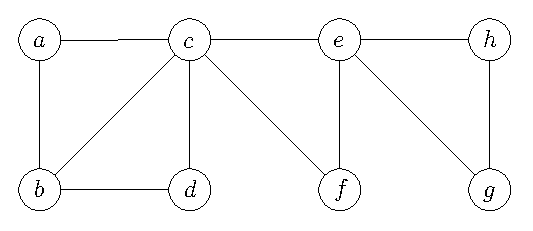
\includegraphics[width=0.5\textwidth]{fig_2a.eps}
\end{center}

\smallskip
\begin{enumerate}[(i)]
\item (3.5 points)
Draw the breadth-first search tree for G assuming that the search starts at node $a$ and that ties among nodes are broken according to the alphabetical order.


\begin{proof}[Solution]
I've done BFS adding all children starting from the left and moving up.
 
So In a stack starting at a 
$
a = \begin{bmatrix}
b\\c
\end{bmatrix}
$
poping b gives us a stack 
$
ab = \begin{bmatrix}
c\\d
\end{bmatrix}
$

 \begin{align*}
now \; abc &= \begin{bmatrix}
d\\e\\f
\end{bmatrix}\\
abcd &= \begin{bmatrix}
e\\f
\end{bmatrix}\\
abcde &= \begin{bmatrix}
f\\g\\h
\end{bmatrix}\\
abcdef &= \begin{bmatrix}
g\\h
\end{bmatrix}\\
abcdefg
\end{align*}


\end{proof}

\vfill
\item (3.5 points)
Draw the depth-first search tree for G assuming that the search starts at node $a$ and that ties among nodes are broken according to the alphabetical order.


\begin{proof}[Solution].\\
there are 4 depths in this graph. d,f,e are one depth sorry for the picture. 

	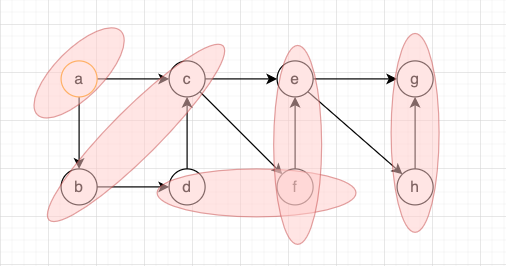
\includegraphics[scale=.5]{q2show.png}

\end{proof}

\end{enumerate}



\newpage
\item (4 points)
Draw two topological orderings of the following graph.

\vspace{2mm}

\begin{center}
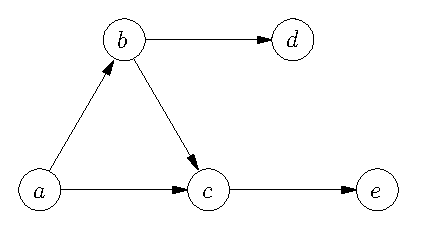
\includegraphics[width=0.4\textwidth]{fig_2b.eps}
\end{center}
$
A. \begin{bmatrix}
	a & b & c & d & e
\end{bmatrix}\\
B. \begin{bmatrix}
	a & b & d & c & e
\end{bmatrix}
$
\smallskip
\smallskip

\item (4 points)
State all strongly connected components of the following graph (in the form of $\{a,b,...\}$, $\{...\}$, ... ).
\vspace{2mm}

\begin{center}
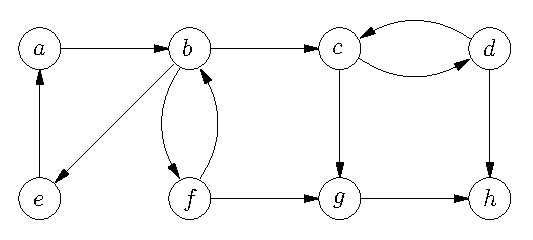
\includegraphics[width=0.5\textwidth]{fig_2c.eps}
\end{center}



\end{enumerate}
\begin{align*}
& [a,b,e], [f,b], [c,d]\\
&[g], [h], [a,b,e,f]
\end{align*}

\newpage



\problem{Graphs}{15}

\begin{enumerate}[(a)]
\item (7 points)
Let $G= (V,E)$ be a directed graph.
The length of each edge in $G$ is one.
Define $G^{2} = (V,E')$ as follows: for vertices $u,v \in V$,
$(u,v) \in E'$ if there is a path of length two between $u$ and $v$ in $G$.
Suppose that a directed graph is given as adjacency matrix.
Design an algorithm to compute $G^2$.
Derive the running time of your algorithm. 

\begin{algorithm}[H]
\Fn(){groundvertices}{
\SetAlgoLined
\SetNoFillComment
\If{ V = 1x1 array}{
	return empty 1x1 matrix;
}
// do matrix multiplication \;
Graph c\;
\For {i = 0 to V[G]}{
   \For{j = 0 to V[G]}{
    	\For{k = 0 to V[G]}{
            $ c[i, j] = c[i, j] + c[i, k] \cdot c[k, j]$\;
       }
   }
}
\Return{c}
}
\end{algorithm}
\begin{proof}
Nested loops from 0 $\rightarrow$ V length means that the time complexity $V\cdot V \cdot V = O(V^3)$

\end{proof}

\newpage

\item(8 points)
Given a directed graph $G = (V, E)$ with $|V| = m$ and $|E| = n$, a vertex $v$ is said to be a ground vertex if there is a path from every other vertex of the graph to $v$.
Note that a graph may have multiple ground vertices.  
Given the adjacency list representation of $G$, design an algorithm to find a ground vertex if one exists. 
If the graph has multiple ground vertices, then it suffices to output one of them.
Derive the running time of your algorithm.
Your grade will depend on the efficiency of your algorithm. 

\begin{algorithm}[H]
\Fn(){groundvertices}{
\SetAlgoLined
\SetNoFillComment
\If{Size of V = 1}{
	return V[0];
}
List  = size of V\;
\For{ i : V[i]}{
	DFS(V,V[i])\;
	\For{ i : list[i]}{
		\If{V[i] = visited}{
			V[i] = unvisited\;
			list[i]++\;
		}
	}
}
\For{ i : list[i]}{
	\If{list[i] = V.length}{
		\Return{i}\;
	}
}
\Return{-1}
}
\end{algorithm}
\begin{algorithm}[H]
\Fn(){DFS( V , i )}{
\SetAlgoLined
\SetNoFillComment
\For{i : threw all adj edges }{
	\If{visited[i] == false}{ 
		mark node as visited\;
		DFS(V,adj.edge)	\;
	}
}
	\Return{current index}\;
}
\end{algorithm}

\begin{proof}
Efficiency of your algorithm is baced on DFS which we know is O(V+E). V number of calls to DFS are done to astablish a list of size v that shows how much vertexs have access to that node. as the end if V DFS calls I search the list for a number of v connections. doing so is time O(V) this gives us a running time for $O(V(V+E) + V) = O(V^2+VE)$ now we know that E is equal to V(V-1) meaning that $O(V^2+VE) = O(V^2+V(V(V-1)))=O(V^2+V^3-V^2) = O(V^3) $ oof
\end{proof}

\end{enumerate}

\newpage

\problem{Dvide and Conquer}{15}

Suppose that $\mathtt{Subroutine}(A,B)$ takes as argument two arrays of integers $A$, $B$ and returns an array. 
The running time is $O(n)$, where $n$ is the number of elements of $A$ plus the number of elements in $B$.
The above algorithm is used in the recursive \Mystery algorithm given below.

%\begin{verbatim}
%1 Mystery(A) 					
%2 if $n = 1$, return A[0].
%3 $A_{1} = A[0]\ldots A[n/2]$ // The first half of $A$.
%4 $A_{2} = A[n/2]\ldots A[n]$ // The second half of $A$.
%5 $A_{3} = A[n/4]\ldots A[3n/4]$ // The middle half of $A$..
%6 $B_1 = Mystery(A_1)$.
%7 $B_2 = Mystery(A_2)$.
%8 $B_3 = Mystery(A_3)$.
%9 $a =$ Subroutine($B_1$, $B_2$).
%10 $b =$ Subroutine($B_2$, $B_3$).
%11 return $a + b$. // Constant ($O(1)$) time
%\end{verbatim}

\begin{algorithm}[H]
\Fn(){\Mystery{$A$}}{
%\KwIn{An array of integers $A = \langle A[0], A[1], \dots , A[n] \rangle$.}
%\KwOut{The adjacency list representation of $\Grev$.}
\SetAlgoLined
\SetNoFillComment
\DontPrintSemicolon
	\If{$n == 1$}{
		\Return{$A[0]$}
	}
	$A_{1} = \langle A[0]\ldots A[n/2-1] \rangle$  \tcp*{The first half of $A$.}
	$A_{2} = \langle A[n/2]\ldots A[n-1] \rangle$  \tcp*{The second half of $A$.}
	$A_{3} = \langle A[n/4]\ldots A[3n/4-1] \rangle$  \tcp*{The middle half of $A$.}
	$B_1 = \Mystery(A_1)$ \\
	$B_2 = \Mystery(A_2)$ \\
	$B_3 = \Mystery(A_3)$ \\
	$C_1 = \Subroutine(B_1, B_2)$ \\
	$C_2 = \Subroutine(B_2, B_3)$ \\
	$C_3 = \langle C_1[0] \ldots C_1[n/2-1], C_{2}[n/2]\ldots C_{2}[n-1] \rangle$ \tcc*{Concatenating 1st half of $C_{1}$ and 2nd half of $C_{2}$}
	\Return{$C_3$} \tcp*{Constant $O(1)$ time.}
}
%\textcolor{blue}{\caption{$\MergeSort(A)$}\label{alg:MergeSort}}
\end{algorithm}

Let $T(n)$ denote the running time of Mystery on an array of n elements.

\pagebreak
\begin{enumerate}[(a)]

\item(7 points) Write the recurrence equation for $T(n)$. (Hint: You may use the following facts: (1) the formula for the geometric series $\sum\limits_{k=0}^{m-1} ar^k = a\left( \frac{r^m - 1}{r - 1}\right)$, for any $r \neq 1$; and (2) $a^{\log_b n} = n^{\log_b a}$.)\\

\begin{proof}[Solution]
	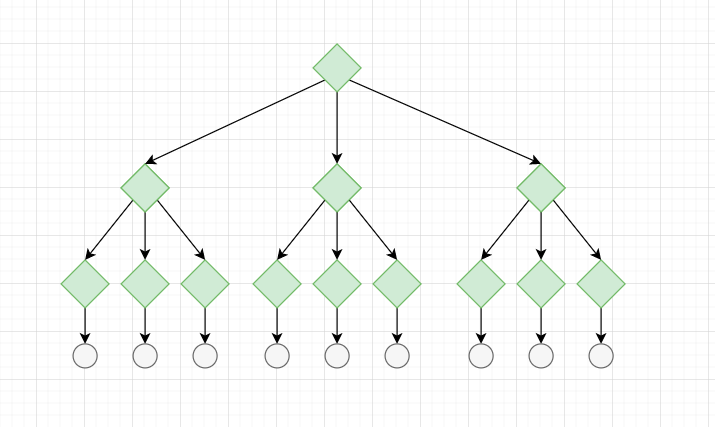
\includegraphics[scale=.5]{q4graph.png}
	
	by following the algoritm we can see that the base case is T(1) = 1 \\
T(2) = a split of 3 nodes off of origonal = 3+1 = 4
T(3) = 3 splits of T(2) giving us 9 children of T(2) = 3+9+1 =13
Now in this recursive function T(n/3) will give the recurence. 

This gives us the start to our equation T(n) = aT(n/3) + b
by spliting the array into 3 parts this gives us a = 3
now$ C_1,C_2,C_3$ all run in n times giving us T(n) = 3T(n/3)+3n
\end{proof}
\newpage

\item(8 points) What is the running time of \Mystery on $n$-element array? Justify your answer. You are not allowed to use the Master Theorem.
\begin{proof}[image].\\
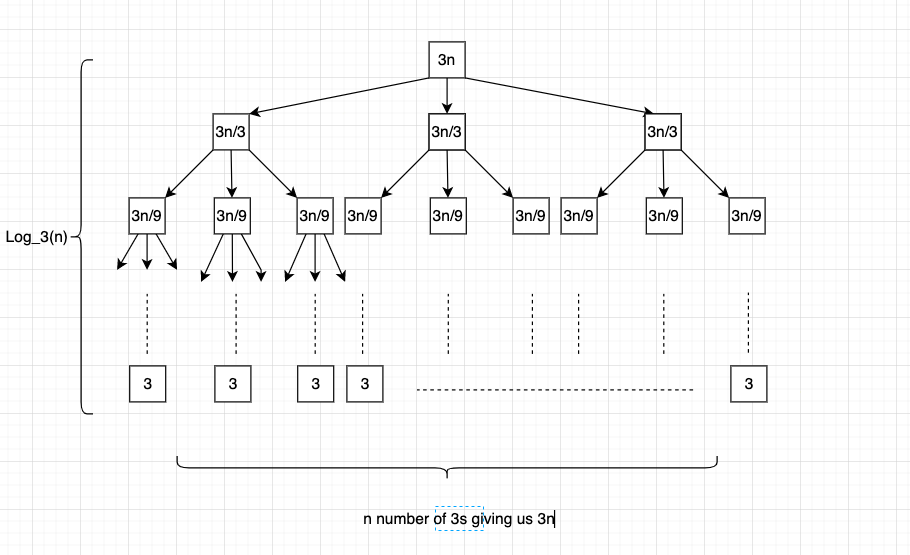
\includegraphics[scale=.5]{q4b.png}
\begin{proof}
By recursion we can see that the total is $3nlog_3n + 3n$ this in turn is $O(nlogn)$

\end{proof}
The Substitution Method

Recurrence:T(n) =3T(n/3) +3n, with T(1) = 1.

Guess:T(n)$\leq c(n/3)log_3(n/3)$, for some constant c.

Consider $n > 1$

\begin{align*}
T(n) &= 2T(n/2)+3n\\
&\leq 2(c(n/3)log_3(n/3)) + 3n\\
&\leq 2cnlog_3n - 2nlog_33 + 3n = 2cnlog_3n - 2n + 3n \\
&=  2cnlog_3n +n
\end{align*}
thus T(n) =$O(nlogn).$


\end{proof}


\end{enumerate}

\newpage

\problem{Bonus Question:}{10}

Suppose that $A$ is an array of natural numbers, i.e., elements in $\{1,2,3,\ldots\}$. 
An element $x$ in $A$ is called a \textbf{majority element} if \textit{strictly} more than half the array cells contain value $x$. For example, $1$ is the majority element of $[1,2,1,1]$. Suppose that the following algorithm is available to us:

\smallskip
\isMajElement($B$, $x$): Takes in an array $B$ of natural numbers and a natural number $x$ and returns true if and only if $x$ is the majority element in $B$. 
The running time is $O(n)$, where $n$ is the length of $B$.

\begin{enumerate}[(a)]
\item(4 points) Complete the following \textit{recursive} algorithm which takes in an array $A$ of natural numbers, and returns the majority element $x$ if there is one, and $-1$ otherwise. Note: No points will be given for non-recursive solutions. ({\em Hint:} In order for some element x to be a majority element in an array, it must be a majority element of either the left half, the right half, or both.) 

%\smallskip
%\begin{verbatim}
%findMajority(A){
%    if(|A| == 1): return A[0]
%    \\YOUR PSEUDOCODE HERE
%}
%\end{verbatim}


\smallskip
\begin{algorithm}[H]
\Fn(){\findMajority{$A$}}{
%\KwIn{An array of integers $A = \langle A[0], A[1], \dots , A[n] \rangle$.}
%\KwOut{The adjacency list representation of $\Grev$.}
\SetAlgoLined
\SetNoFillComment
\DontPrintSemicolon
	\If{$(|A| == 1)$}{
		\Return{$A[0]$}
	}
	size = n/2\;
	$x_1 =  findMajority([A[0],\cdots, A[n/2]]$\\
	$x_2 = findMajority([A[n/2]+1,\cdots,A[n]]$\\
	\If{$x_1 = x_2$}{
			\Return $x_1$\;
	}
	$SubMajority_1 =isMajElement(A,x_1)$\;
	$SubMajority_2 =isMajElement(A,x_2)$\;
	
	\If{$SubMajority_1$}{
		\Return $x_1$\;
	}
	\If{$SubMajority_2$}{
		\Return $x_2$\;
	}
	\Return -1\;
}
%\textcolor{blue}{\caption{$\MergeSort(A)$}\label{alg:MergeSort}}
\end{algorithm}


\newpage

\item(3 points) What is the recurrence equation of your algorithm? (No justification required, just write the recurrence).

$T(n) = 2T(n/2) + n$\\
\vfill

\item(3 points) What is the running time of your algorithm? (No justification required, just write the running time in Big-O notation)

$O(nlogn)$
\vfill

\end{enumerate}

\newpage
\section*{Scratch Paper}

\pagebreak
\section*{Scratch Paper}

\pagebreak
\section*{Scratch Paper}


\pagebreak
\section*{Scratch Paper}


%\vfill

\end{document}
